\documentclass[12pt]{article}
\usepackage[a4paper]{geometry}
\usepackage[utf8]{inputenc}
\usepackage{fancyhdr}
\usepackage{lastpage}
\usepackage{graphicx, wrapfig, subcaption, setspace, booktabs}
\usepackage{graphicx}
\usepackage[T1]{fontenc}
\usepackage[font=small, labelfont=bf]{caption}
\usepackage[protrusion=true, expansion=true]{microtype}
\usepackage[english]{babel}
\usepackage{sectsty}
\usepackage{url, lipsum}
\usepackage[T1]{fontenc}
\usepackage{icomma}
\usepackage{siunitx}
\usepackage{ragged2e}
\usepackage{amsmath}
\usepackage{comment}
\usepackage{enumerate}
\usepackage{anysize}


\newcommand{\HRule}[1]{\rule{\linewidth}{#1}}
\onehalfspacing
\setcounter{tocdepth}{5}
\setcounter{secnumdepth}{5}

\begin{document}

\begin{titlepage}

\title{ \normalsize 
        \begin{center}
        
\includegraphics[height=6cm]{logo.png}
        \end{center}
        \LARGE \textsc{\textbf{Universidad De Sonora}} \\ \bigskip
		\Large División de Ciencias Exactas y Naturales \\
        Licenciatura en Física \\ \bigskip
        \bigskip
        Física Computacional I
		\\ [0.1cm]  
		\HRule{2pt} \\
		\Large \textbf{{Actividad 8}} \\
        \textit{\textbf{"Oscilador de Van de Pol"}}
		\HRule{2pt} \\
		\normalsize \vspace*{0.001\baselineskip}}
        
\date{\bigskip \Large Hermosillo, Sonora  \hspace*{\fill}  12 de Abril de 2018}

        
\author{
		\Large\textbf{ Michelle Contreras Cossio} \\ \bigskip
        \\ \bigskip
       \Large Profr. Carlos Lizárraga Celaya}
       \end{titlepage}
       \maketitle
       

\newpage
\pagestyle{plain}

\section{Introducción - Antecedentes}

El siguiente reporte presenta la actividad 8, realizada durante esta semana sobre el modelo de Van der Pol, un oscilador no conservativo con amortiguamiento no lineal, presentando la teoría detrás de este en la siguiente sección. Además, se presentan las gráficas realizadas para ilustrar este movimiento oscilatorio, así como el proceso que se realizó para poder llegar a estas. \\

Durante esta actividad se trabajó haciendo uso de Python mediante el Jupyter Lab, utilizando varias de las bibliotecas que este lenguaje nos presenta, como son Numpy, Matplotlib, Pylab y con particular enfoque en odeint de Scipy, que ya fue utilizado en prácticas anteriores. \\

\section{Modelo de Van der Pol}

Como se mencionó anteriormente, el modelo de Van der Pol es un oscilador no conservativo con amortiguamiento no lineal, que obedece la siguiente ecuación diferencial:

\begin{equation}
\frac{d^2x}{dt^2} -\mu (1-x^2) \frac{dx}{dt}+x=0
\end{equation}

Donde x es la posición en función del tiempo t y $\mu$ es un parámetro escalar que indica la no linealidad y fuerza del amortiguamiento

\subsection{Historia}

El oscilador de Van der Pol fue propuesto por el físico e ingeniero eléctrico alemán Batlthasar Van der Pol, mientras trabajaba para la empresa alemana Philips. \\

Lo que lo llevó a encontrar este modelo fue que encontró oscilaciones estables, llamadas posteriormente oscilaciones de relajación y actualmente se utilizan conocidas como ciclos límite de los circuitos eléctricos.  \\

Cuando los circuitos se llevaban a su ciclo límite, la señal arrastraba consigo a la corriente, esto lo publicó junto con si colega van der Mark en la revista Nature. Posteriormente se logró descubrir que esto se debía al caos determinista \\

La ecuación de Van der Pol se ha utilizado en muchos fenómenos tanto físicos como de otras ciencias como la biología, como fue el caso de Fitzhugh y Nagumo, para modelar el potencial de acción de las neuronas. Otro ejemplo es para modelar dos placas tectónicas en una falla. 

\subsection{Forma bidimensional}

Para lograr representarla con dos ecuaciones de primer orden, o en su forma bidimensional, se utiliza la transformación de Liénard $y=x-x^3/3 -\dot{x}/\mu$. Convirtiendo la ecuación (1) de la siguiente forma:

\begin{equation}
\dot{x}=\mu (x-\frac{1}{3}x^3 -y)
\end{equation}
\begin{equation}
\dot{y}=\frac{1}{\mu}x
\end{equation}

O utilizando la transformación $y=\dot{x}$ el sistema queda:

\begin{equation}
\dot{x}=y
\end{equation}
\begin{equation}
\dot{y}=\mu(1-x^2)y-x
\end{equation}

\subsection{Resultados para el oscilador no forzado}

Las oscilaciones no forzadas indican $\mu=0$ y la ecuación (1) queda de la siguiente forma:

\begin{equation}
\frac{d^2x}{dt^2}+x=0
\end{equation}

Formando un oscilador armónico simple con conservación de energía.\\

Cuando $\mu >0$, el sistema entra al ciclo límite, cerca del origen el sistema es inestable, lejos de este es amortiguado.\\

Este oscilador no tiene una solución analítica exacta.

\subsection{Hamiltoniano para el oscilador de Van der Pol}

También se puede escribir el oscilador de Van der Pol en términos del Hamiltoniano independiente del tiempo, aumentando el sistema a uno de cuatro dimensiones.Para poder encontrar el Hamiltoniano, primero escribimos el modelo como un sistema de ecuaciones de segundo orden:

\centering $\ddot{x}-\mu(1-x^2)\dot{x}+x=0$\\
$\ddot{y}+\mu(1-x^2)\dot{y}+y=0$ \\

\justify
De las cuales podemos obtener el Hamiltoniano de la siguiente manera: \\

\centering $H(x,y,p_x, p_y)=p_x p_y +xy -\mu(1-x^2)yp_y$ \\

\justify
Donde $p_x$ y $p_y$, son los momentos respectivos a $x$ y $y$.

\subsection{Circuitos eléctricos}

Van der Pol construyó el oscilador con un triodo o tetrodo. Para poder involucrar el modelo con circuitos eléctricos, se añaden la corriente y el voltaje de la siguiente estructura: $i= \phi(v)= \gamma v^3 -\alpha v$. Con esto el oscilador queda de la siguiente manera: \\

\centering $\ddot{V}-\frac{1}{C}(\alpha -3\gamma V^2)\dot{V}+ \frac{1}{LC}V=0$

\justify

Que puede ser reescrita a la ecuación (1) del oscilador de Van der Pol original utilizando las transformaciones apropiadas. 

\subsection{Oscilador de Van der Pol Forzado y Caos Determinista}

El oscilador de Van der Pol forzado utiliza la función original añadiéndole una fuerza externa senoidal, resultando ahora el modelo de la siguiente forma:

\begin{equation}
\frac{d^2x}{dt^2} -\mu (1-x^2) \frac{dx}{dt}+x-Asin(\omega t)=0
\end{equation}

Donde $A$ es la amplitud de la onda de la fuerza y $\omega$ es la velocidad angular de esta misma.\\

Van der Pol, en conjunto con Van der Mark, estudiaron un circuito eléctrico conectándolo a unos receptores de teléfono, del que escucharon sonidos irregulares, pero no fue hasta después de que Ueda y Lorenz desarrollaran teoría sobre los atractores caóticos, que se logró identificar que lo que escucharon era el caos determinista.

\clearpage

\section{Exploración de las soluciones del modelo en el Espacio Fase}

En esta sección se demuestra por medio de gráficas, como independientemente de las condiciones iniciales, en el espacio fase siempre se llegará al mismo ciclo límite. Nota: el código utilizado se muestra en la siguiente sección, análogo al correspondiente a la gráfica \#1. \\

Todas las gráficas cuentan con $\mu$=2.0.

\begin{figure}[h!]
\begin{subfigure}{.55\textwidth}
\centering
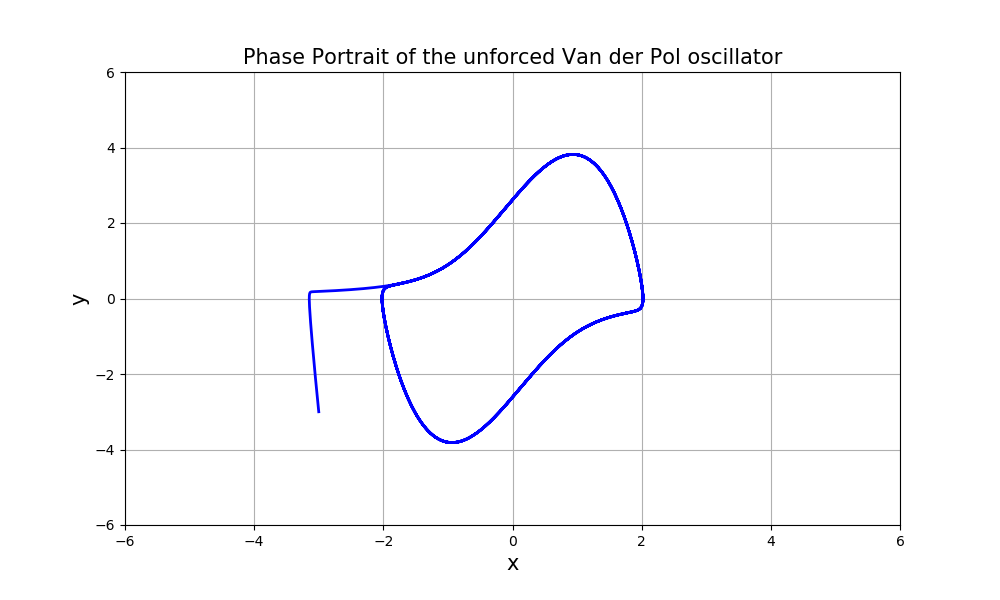
\includegraphics[width=1\linewidth]{CI1.png}
\caption{Condiciones iniciales: x=-3.0, y=-3.0}
\end{subfigure}
\begin{subfigure}{.55\textwidth}
\centering
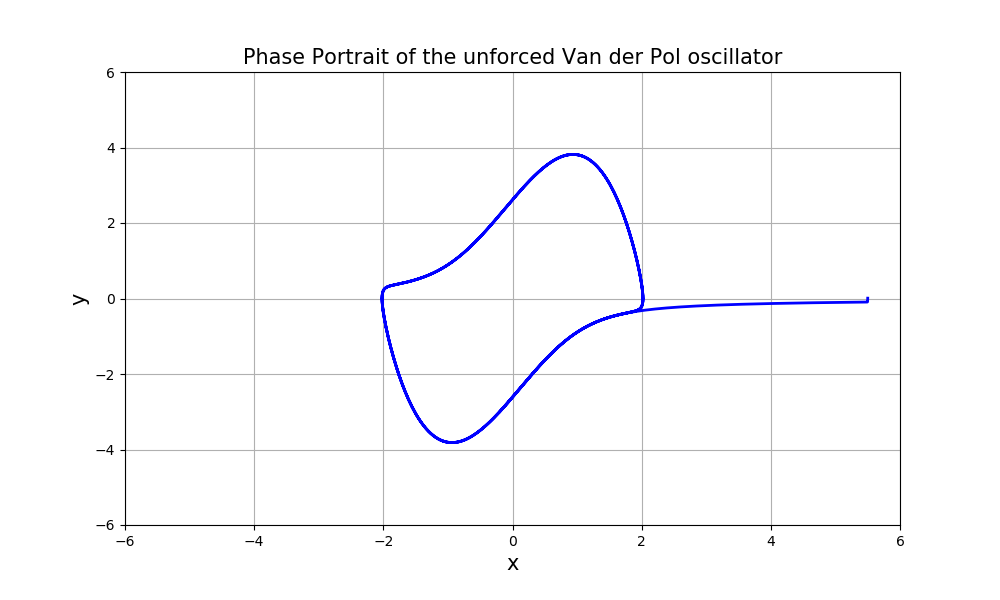
\includegraphics[width=1\linewidth]{CI2.png}
\caption{Condiciones iniciales: x=5.5, y=0.009}
\end{subfigure}
\begin{subfigure}{.55\textwidth}
\centering
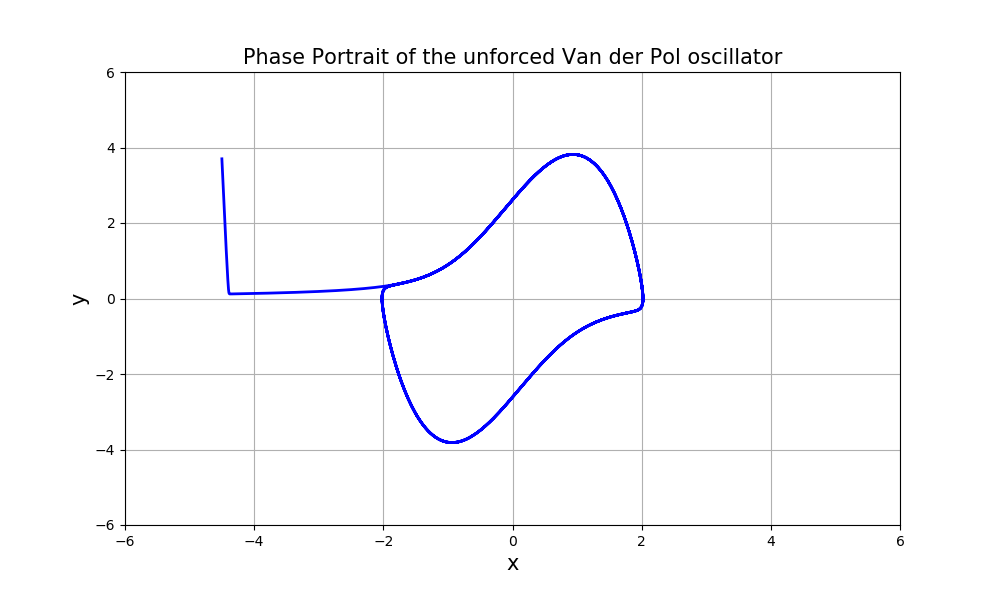
\includegraphics[width=1\linewidth]{CI3.png}
\caption{Condiciones iniciales: x=-4.5, y=3.5}
\end{subfigure}
\begin{subfigure}{.55\textwidth}
\centering
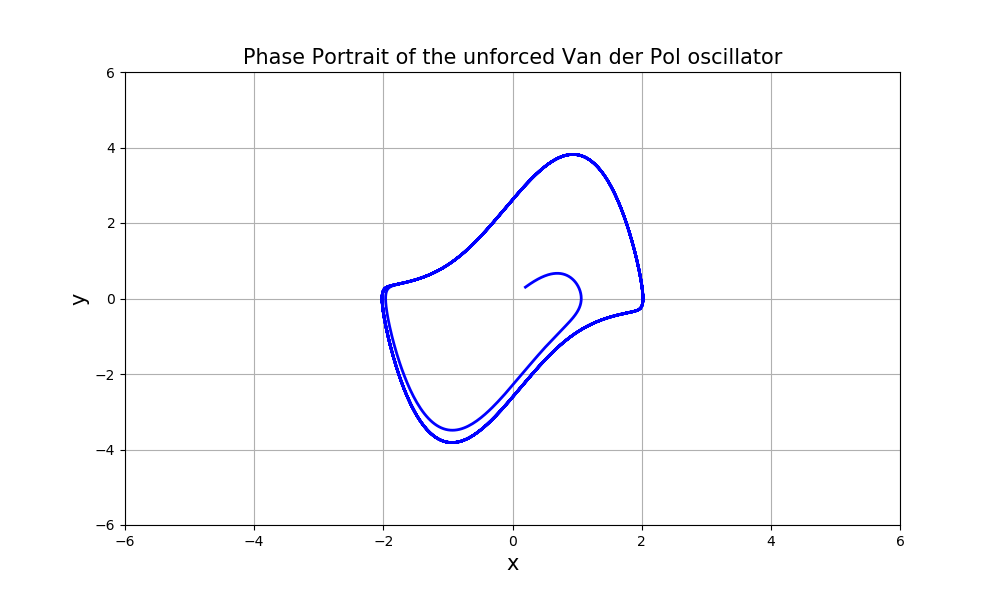
\includegraphics[width=1\linewidth]{CI4.png}
\caption{Condiciones iniciales: x=0.2, y=0.3}
\end{subfigure}
\end{figure}

Como se puede observar, independientemente de las condiciones iniciales que se le inserten, dentro del programa, siempre va a converger al mismo ciclo límite, tal como un atractor. 


\section{Resultados y discusión}

Se reproducieron 4 gráficas contenidas en el artículo de Wikipedia del Oscilador de Van der Pol. En esta sección se muestra el código utilizado para ellas y el resultado obtenido. \\

El código utilizado en las cuatro gráficas es similar:


\begin{enumerate}
\item Primeramente se definió la función de Van Der Pol de la siguiente manera: 

\begin{center}
        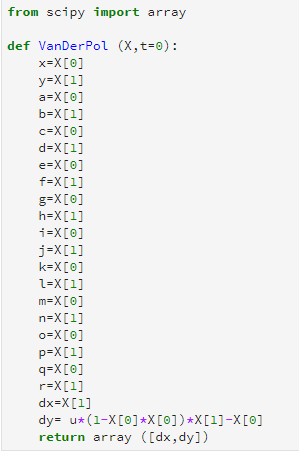
\includegraphics[height=8.7cm]{1.png}
\end{center}

Se utilizaron muchas variables para las diferentes condiciones iniciales que presentan las gráficas. En el caso de la cuarta gráfica únicamente se insertó una pareja de condiciones iniciales (x,y) y los valores de dx y dy cambian al insertar la fuerza senoidal a la ecuación.

\item Posteriormente se importaron las bibliotecas necesarias y se dieron las condiciones iniciales, además de la solución a la ecuación diferencial con la función odeint: 
\begin{center}
        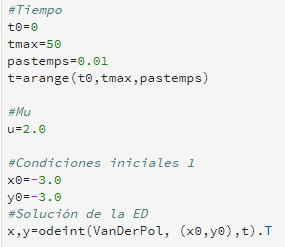
\includegraphics[height=5cm]{2.png}
\end{center}
Estas varían según la gráfica que se desea representar, pero el formato es el mismo, en las gráficas \#1 y \#2 se tienen cuatro y diez condiciones iniciales, respectivamente. 
\item Finalmente, se realizó el plot de cada gráfica
\end{enumerate}

\begin{itemize}
\item \textbf{Gráfica \#1: Espacio fase de un oscilador de Van der Pol no forzado, mostrando el ciclo límite y el campo de direcciones}

En esta gráfica, además del código mencionado anteriormente, se utilizó lo siguiente:

\begin{center}
        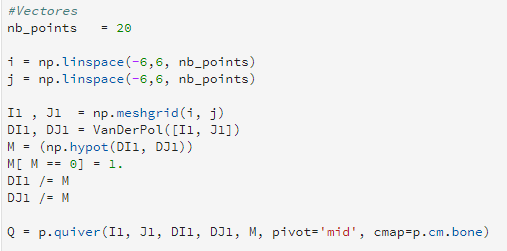
\includegraphics[height=5cm]{3.png}
\end{center}

Que nos permite realizar el campo vectorial, resultando el plot:

\begin{center}
        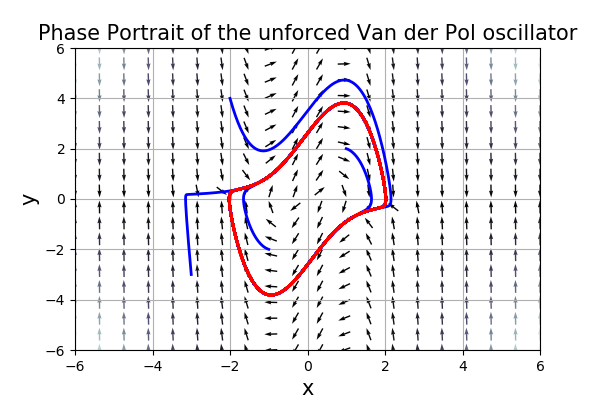
\includegraphics[height=7cm]{Graf1.png}
\end{center}

Esta gráfica preserva la misma idea de que independientemente de las condiciones iniciales, se llega al mismo ciclo límite, presentado en las cuatro gráficas de la sección anterior. Además de eso, se añade el campo vectorial que nos indica hacia donde se dirige la función. \\

Se muestra, en una sola imagen, cuatro condiciones iniciales distintas (azul) que convergen al mismo ciclo límite (rojo). Todas cuentan con $\mu$=2.0.

\clearpage
\item\textbf{Gráfica \#2: Evolución del ciclo límite en el espacio fase, con $\mu$ variable.}

En esta gráfica, como se mencionó, se realizó 10 veces el paso 2, de manera que en una sola imagen se presentan 10 gráficas con diferentes valores para $\mu$, pero con las posiones iniciales constantes (-2,0):

\begin{center}
        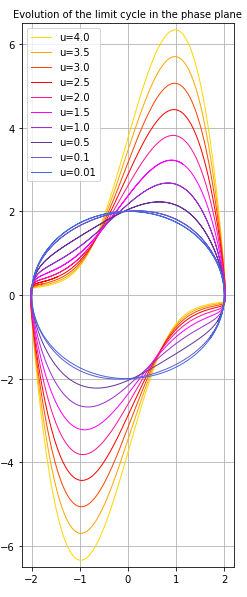
\includegraphics[height=15cm]{Graf2.png}
\end{center}

Aquí, como en la gráficas anteriores, tenemos el ciclo límite, pero en este caso, lo que varía es $\mu$, las posiciones iniciales son las mismas. Así podemos ver como el ciclo límite se va deformando desde un círculo, hasta una figura más alargada, mientras incrementamos el valor de $\mu$.

\clearpage
\item \textbf{Gráfica \#3: Oscilación relajada en el oscilador de Van der Pol, sin fuerza externa, con valor de amortiguamiento no lineal $\mu$=5}

\begin{center}
        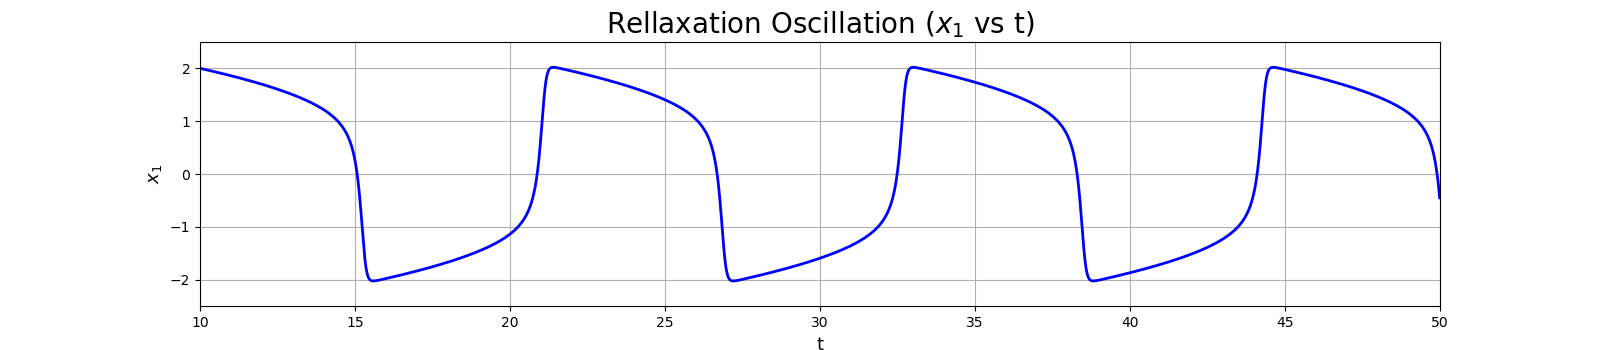
\includegraphics[height=3.5cm]{Graf3.png}
\end{center}

Esta gráfica ya no presenta la posición con respecto a la velocidad, sino, la posición con respecto al tiempo, donde podemos observar que se da una oscilacion, llamada "relajada".

\item \textbf{Gráfica \#4: Comportamiento caótico en el Oscilador de Van der Pol con fuerza externa senosoidal.}

Como se mencionó, para este gráfico de tuvo que definir de nuevo el VanDerPol, para agregar la fuerza externa, además se añadieron los parámetros para la amplitud y frecuencia de la fuerza, con valores de $A=1.2$, $\omega=2\pi /10$, $\mu=8.53$. Además de eso, no hubo ninguna otra variación con respecto a las otras gráficas. 

\begin{center}
        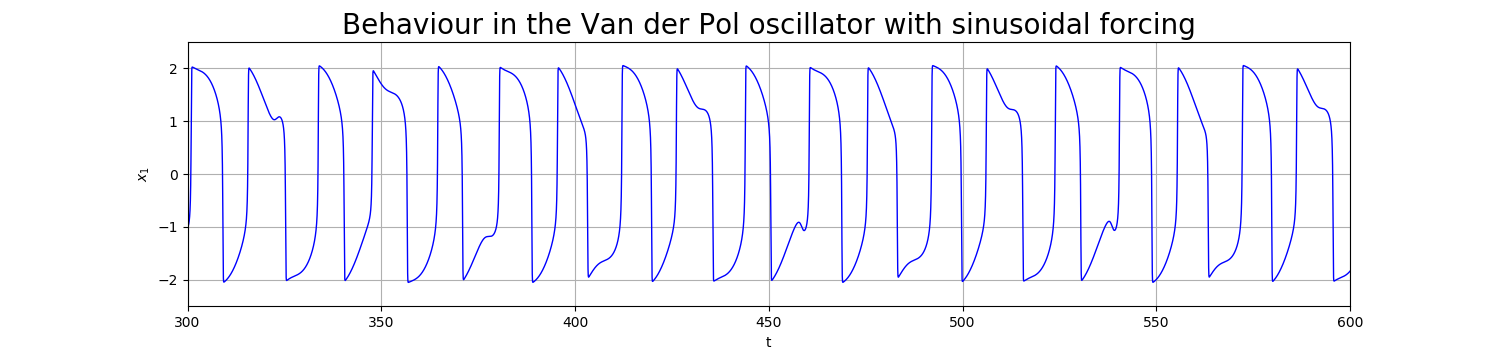
\includegraphics[height=4cm]{Graf4.png}
\end{center}
\end{itemize}

Aquí podemos comparar esta con la gráfica anterior y ver el efecto que tiene agregar la fuerza senosoidal al oscilador, ya no tenemos un movimiento tan "suave" o "relajado". 
\section{Conclusiones del estudio}

Fue realmente satisfactorio saber que contamos con herramientas, como lo es Python, que nos permitan modelar o reproducir con gran precisión ecuaciones como esta. Esto nos abre una gama de posibilidades muy extensa, con la cual no nos tenemos que conformar con las gráficas que encontramos en línea, sino que crear una por nuestra cuenta e incluso modificarlas o "jugar" con ellas.\\ 

La conclusión a la que se puede llegar, con respecto a la teoría, recae en la importancia que tiene el coeficiente no lineal, agregado a un oscilador simple, puede llevarnos a este comportamiento tan particular como es el caos. Poniéndolo en otro contexto o a manera de moraleja, un pequeño error o cambio, nos puede llevar al caos.


\section{Bibliografía}

\begin{itemize}
\item Van der Pol oscillator (2018). Consultado: 11 de Abril del 2018, de Wikipedia. Sitio web: https://en.wikipedia.org/wiki/Van\_der\_Pol\_oscillator
\item Van der Pol oscillator (2007). Takashi Kanamaru. Consultado: 11 de Abril del 2018, de Scholarpedia. Sitio web:  http://www.scholarpedia.org/article/Van\_der\_Pol\_oscillator
\end{itemize}

\section{Apéndice}

\begin{enumerate}
\item Este ejercicio pareciera similar al desarrollado en las actividades 6 y 7. ¿Qué aprendiste nuevo?

A hacer el campo vectorial que muestre hacia donde se dirige la función graficada. 

\item ¿Qué fue lo que más te llamó la atención del oscilador de Van der Pol?

Me gustó el reto, ya que no era simplemente copiar un código y entenderlo, creo que en esta práctica pude realmente entender lo que hice en las dos anteriores.

\item Has escuchado ya hablar de caos. ¿Por qué sería importante estudiar este oscilador?

Había escuchado hablar, pero no estoy muy familiarizada con el término, siento que es bastante interesante algo que se comporte de esta manera, como el oscilador de Van der Pol, donde independientemente de las condiciones iniciales, regresa al ciclo límite.

\item ¿Qué mejorarías en esta actividad?

Nada, ha sido de mis favoritas.

\item ¿Algún comentario adicional antes de dejar de trabajar en Jupyter con Python?

:(, no sabía que era la última vez que ibamos a trabajar con Python, quisiera seguir usándolo, siento que podemos aprender mucho más.

\item Cerramos la parte de trabajo con Python ¿Que te ha parecido?

Me gustó mucho y más que fortran, siento que es un lenguaje que puede aprender cualquiera, por la cantidad de recursos que hay en línea y porque es gratuito utilizarlo en jupyter lab.

\end{enumerate}


\end{document}